\documentclass[aspectratio=169,11pt]{beamer}
\usepackage{beamerucad}
\usepackage{listings}
\definecolor{ckw}{HTML}{2563AB}\definecolor{cst}{HTML}{2E8B57}\definecolor{ccm}{HTML}{8A8F98}
\lstdefinestyle{jv}{language=Java,basicstyle=\ttfamily\footnotesize,
 keywordstyle=\color{ckw}\bfseries,stringstyle=\color{cst},commentstyle=\color{ccm}\itshape,
 showstringspaces=false,columns=fullflexible,keepspaces=true,
 backgroundcolor=\color{ucadband!8},frame=leftline,framerule=2.5pt,rulecolor=\color{ucadband},
 xleftmargin=8pt,aboveskip=3pt,belowskip=1pt,basewidth=0.5em}
\lstset{style=jv}
\title{Architectures Logicielles — Séance 3}
\subtitle{Le monolithe modulaire : des frontières entre les métiers, vérifiées par un test}
\author{Dr. El Hadji Bassirou TOURÉ}
\institute{Département de Mathématiques et Informatique\\ Faculté des Sciences et Techniques\\ Université Cheikh Anta Diop de Dakar}
\date{}
\setucadfoot{Architectures Logicielles --- Séance 3 \quad\textbullet\quad Dr. El Hadji Bassirou TOURÉ --- DMI/FST/UCAD}
\graphicspath{{figs/}}
\begin{document}

\begin{frame}[plain,noframenumbering]\titlepage\end{frame}

\begin{frame}{Objectifs de la séance}
\begin{ucaddef}[Contenu]
{\small L'hexagone du Lab 2 protège le métier de la technique — mais tous les métiers de SénResto vivent dans le \emph{même} hexagone. Cette séance trace les frontières \textbf{entre les métiers} : les \textbf{bounded contexts}, matérialisés en \textbf{modules} dont \textbf{Spring Modulith} garde les frontières par un simple test, et qui collaborent par \textbf{appels d'API publique} ou par \textbf{événements internes}.}
\end{ucaddef}
\begin{itemize}\small
  \item Découper un domaine en \textbf{bounded contexts} — et savoir où passe le trait.
  \item Structurer un \textbf{module} : API publique au paquetage racine, implémentation cachée dans \texttt{interne/}.
  \item Faire vérifier les frontières \textbf{par le build} : une violation = un test rouge.
  \item Choisir entre \textbf{appel direct} et \textbf{événement} — et publier vos premiers événements métier.
\end{itemize}
\end{frame}

% #####################################################################
\section{La frontière manquante}

\begin{frame}{Un hexagone, cinq métiers}
\begin{ucadpiege}[Le constat]
{\small Ouvrez \texttt{domaine/} : commandes, restaurants, livreurs, notifications y cohabitent librement — demain, le catalogue pourra fouiller les données du paiement sans que rien ne l'en empêche. L'hexagone protège le métier \emph{de la technique} — pas les métiers \emph{les uns des autres}.}
\end{ucadpiege}
\begin{itemize}\small
  \item À 5 classes métier, ce n'est pas grave. À 50, c'est le God controller qui renaît — à l'échelle du domaine entier.
  \item La frontière qui manque n'est pas technique : elle est \textbf{métier}. Où finit « commander » et où commence « payer » ?
\end{itemize}
\begin{ucadret}[Le consensus industriel]
{\small \emph{« Monolith first »} (Fowler) : on structure d'abord le monolithe en \textbf{modules à frontières explicites} — réversible, testable, et meilleur brouillon d'un futur découpage en services... si un jour il se justifie.}
\end{ucadret}
\end{frame}

% #####################################################################
\section{Bounded contexts}

\begin{frame}{Le bounded context}
\begin{ucaddef}[Définition (DDD, version allégée)]
{\small Un \textbf{bounded context} est une zone du domaine à l'intérieur de laquelle les mots ont \emph{un} sens précis et le modèle est cohérent. La frontière passe là où \textbf{le vocabulaire change de sens} — pas là où la technique le suggère.}
\end{ucaddef}
\begin{ucadex}[Le test linguistique, sur SénResto]
{\small Que veut dire « commande » ? Pour \textbf{Commandes} : un panier, un client, un statut. Pour \textbf{Livraison} : une course, une adresse, un ETA. Pour \textbf{Paiement} : un montant à encaisser. Même mot, trois modèles — trois contextes.}
\end{ucadex}
\begin{ucadret}[À retenir]
{\small On ne découpe pas un domaine avec un couteau technique mais avec une oreille : \textbf{écouter où le langage change de sens}.}
\end{ucadret}
\end{frame}

\begin{frame}{Les cinq contextes de SénResto}
{\small\begin{tabular}{p{0.17\linewidth}p{0.40\linewidth}p{0.30\linewidth}}
\toprule
\textbf{Module} & \textbf{Sa responsabilité} & \textbf{Son langage}\\
\midrule
\texttt{catalogue} & les restaurants et leurs plats & plat, prix, spécialité\\
\texttt{commandes} & le cycle de vie d'une commande & statut, quantité, montant\\
\texttt{livraison} & assigner et suivre les livreurs & course, position, ETA\\
\texttt{paiement} & encaisser (mobile money simulé) & transaction, encaissement\\
\texttt{notifications} & prévenir les clients & SMS, destinataire\\
\bottomrule
\end{tabular}}
\vskip4pt
\begin{ucadrec}[Ce n'est pas un hasard]
{\small Cinq contextes, cinq membres par groupe : au Lab 3, \textbf{chacun devient propriétaire d'un module} — de son API publique, de ses internes, de ses frontières.}
\end{ucadrec}
\end{frame}

% #####################################################################
\section{Spring Modulith}

\begin{frame}{Un module : une API publique, des internes cachés}
\centering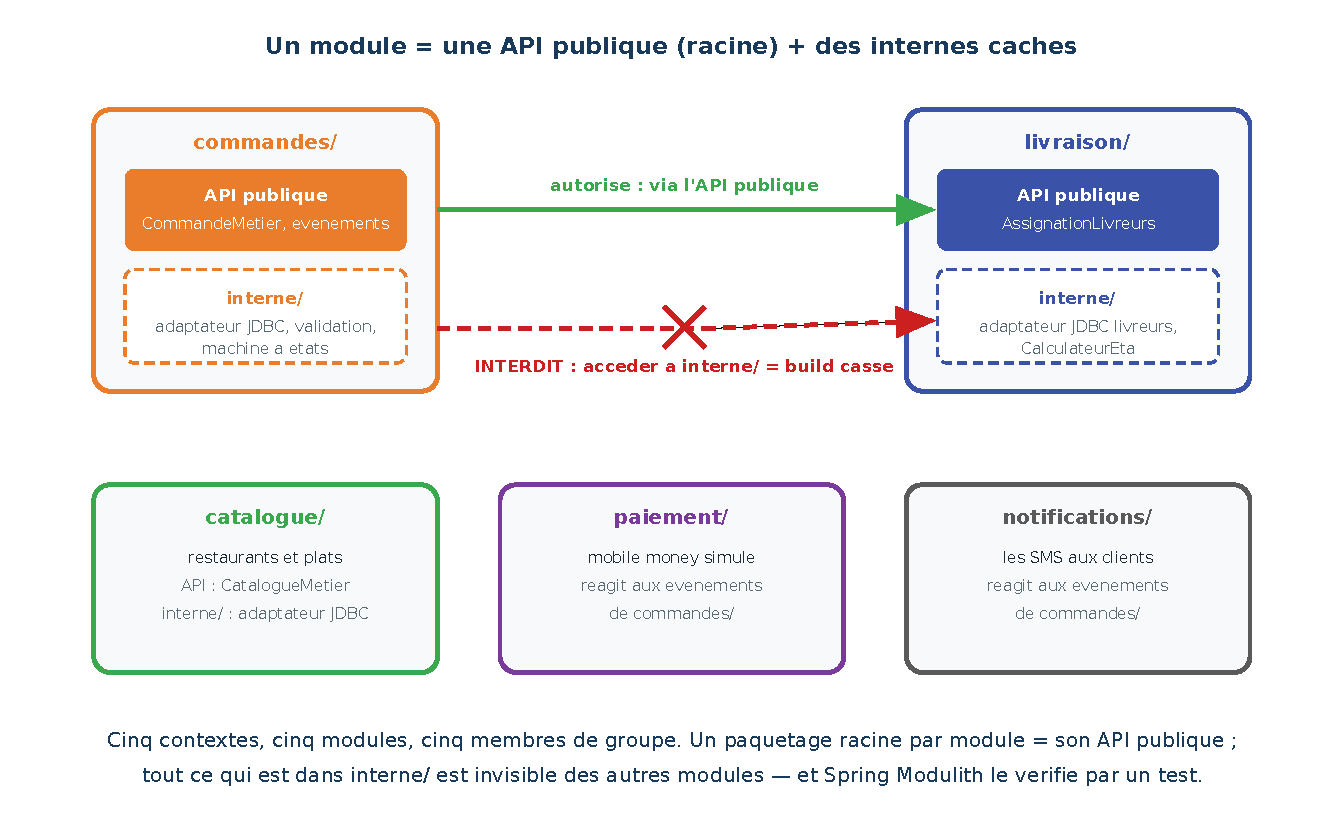
\includegraphics[width=0.72\linewidth]{figG_modules}
\end{frame}

\begin{frame}[fragile]{La convention Spring Modulith}
{\small La règle tient en deux lignes — c'est sa force :}
\begin{lstlisting}
sn/ucad/senresto/
|-- commandes/            <- paquetage direct = MODULE "commandes"
|   |-- CommandeMetier.java     <- racine = API PUBLIQUE du module
|   |-- CommandeConfirmee.java  <- les evenements aussi
|   \-- interne/                <- INVISIBLE des autres modules
|       \-- AdaptateurCommandesJdbc.java
\-- livraison/            <- module "livraison", meme structure
\end{lstlisting}
\begin{itemize}\small
  \item Chaque paquetage directement sous l'application est un \textbf{module} ; seuls les types de son paquetage \emph{racine} sont accessibles aux autres.
  \item Pas de nouveau framework à apprendre : c'est \textbf{une convention de paquetages} — et un gardien qui la fait respecter.
\end{itemize}
\end{frame}

\begin{frame}[fragile]{Le gardien : la frontière vérifiée par un test}
\begin{lstlisting}
class ModulithArchitectureTest {

    @Test
    void lesFrontieresDesModulesSontRespectees() {
        ApplicationModules.of(SenRestoApplication.class).verify();
    }
}
\end{lstlisting}
\begin{itemize}\small
  \item Qu'un développeur importe l'\texttt{interne/} d'un autre module, et ce test devient \textbf{rouge} — le build casse, la violation est nommée, fichier et ligne à l'appui.
  \item L'architecture cesse d'être un dessin sur un slide : elle devient une \textbf{propriété vérifiée en continu}, au même titre qu'un comportement.
\end{itemize}
\begin{ucadret}[À retenir]
{\small La différence entre une convention et une architecture, c'est un \textbf{test qui échoue}. Vous en ferez l'expérience au lab : violation volontaire, build cassé, message lu, violation retirée.}
\end{ucadret}
\end{frame}

% #####################################################################
\section{Les événements internes}

\begin{frame}{Deux façons de collaborer entre modules}
\centering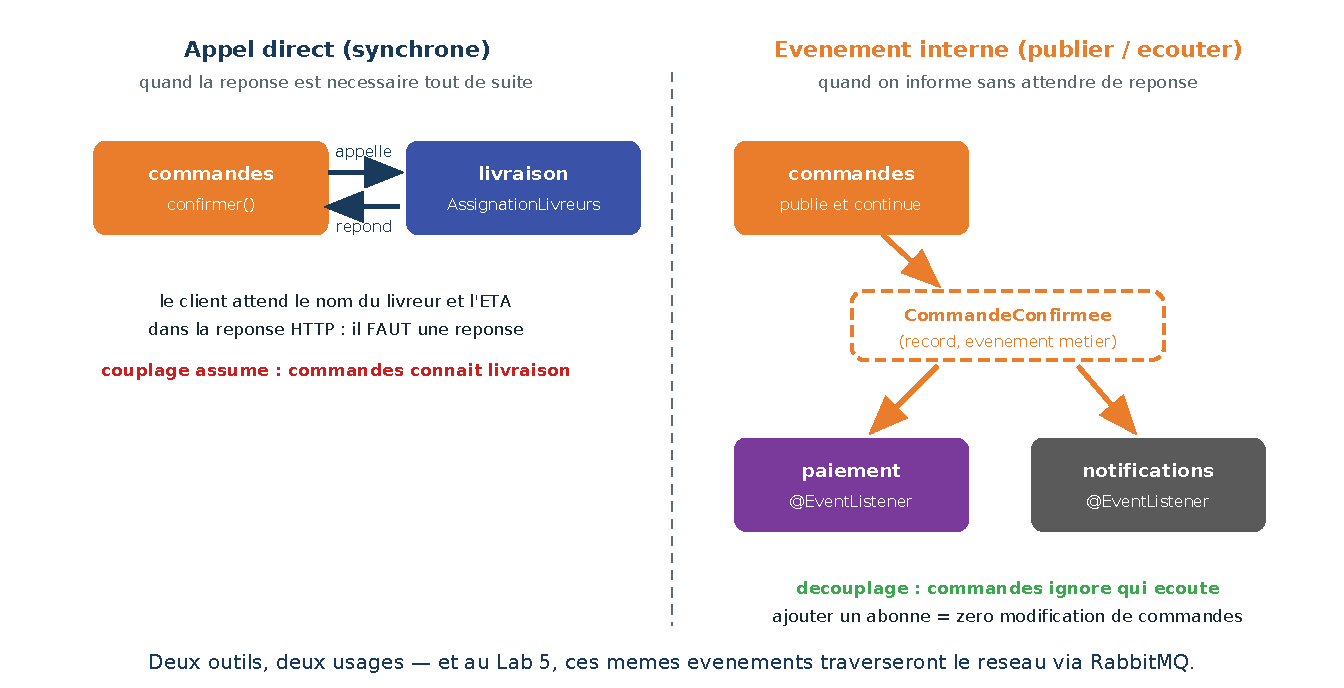
\includegraphics[width=0.74\linewidth]{figH_appel_vs_evenement}
\end{frame}

\begin{frame}[fragile]{Publier un événement métier}
{\small Un événement est un simple \emph{record} — un fait passé, nommé au participe : \emph{la commande a été confirmée}. Il vit dans l'API publique du module qui le publie :}
\begin{lstlisting}
// commandes/CommandeConfirmee.java  (racine du module = public)
public record CommandeConfirmee(long commandeId, String numero,
        String clientTelephone, int montantTotal, String livreurNom,
        int etaMinutes) {}
\end{lstlisting}
\begin{lstlisting}
// Dans CommandeMetier.confirmer(), a la place de l'appel aux notifications :
evenements.publier(new CommandeConfirmee(id, numero, telephone,
        montant, livreurNom, etaMinutes));
\end{lstlisting}
\begin{itemize}\small
  \item \texttt{commandes} annonce un \textbf{fait} et continue sa route : il ignore qui écoute, et n'attend rien de personne.
\end{itemize}
\end{frame}

\begin{frame}[fragile]{Écouter : les abonnés}
{\small Chaque module intéressé déclare un écouteur — dans \emph{ses} murs :}
\begin{lstlisting}
// paiement/interne/EcouteurPaiement.java
@Component
class EcouteurPaiement {

    @EventListener
    void quandCommandeConfirmee(CommandeConfirmee evt) {
        System.out.println("[PAIEMENT] Encaissement mobile money simule : "
                + evt.montantTotal() + " FCFA pour " + evt.numero());
    }
}
\end{lstlisting}
\begin{itemize}\small
  \item \texttt{paiement} est né \textbf{sans modifier une ligne} de \texttt{commandes} — et par défaut ces événements sont \textbf{synchrones} : le comportement observable ne change pas... pour l'instant.
\end{itemize}
\begin{ucadfront}[Le pont vers la séance 5]
{\footnotesize Retenez ces records : au Lab 5, les \emph{mêmes} événements traverseront le réseau via RabbitMQ, vers un service Python. Vous faites déjà de l'event-driven — dans un seul processus.}
\end{ucadfront}
\end{frame}

\begin{frame}{Ce que le modulith achète — et ce qu'il coûte}
\begin{itemize}\small
  \item \textbf{Achète} : des frontières métier vérifiées par le build ; un déploiement qui reste \emph{simple} (un seul processus, une seule BDD, pas de réseau interne) ; des modules extractibles plus tard — le Strangler Fig du Lab 4 cueillera un module déjà découpé ; une documentation d'architecture générable depuis le code.
  \item \textbf{Coûte} : la discipline des paquetages ; des API publiques à concevoir avec soin ; la tentation permanente du raccourci (« juste cet import... ») — que le gardien transforme, précisément, en build cassé.
\end{itemize}
\begin{ucadret}[À retenir]
{\small Le monolithe modulaire offre \textbf{80\,\% des bénéfices d'organisation des microservices pour 20\,\% de leur coût opérationnel}. C'est le point d'équilibre moderne — et le meilleur point de départ pour la suite.}
\end{ucadret}
\end{frame}

% #####################################################################
\section{Le lab}

\begin{frame}{Le chemin du Lab 3}
\centering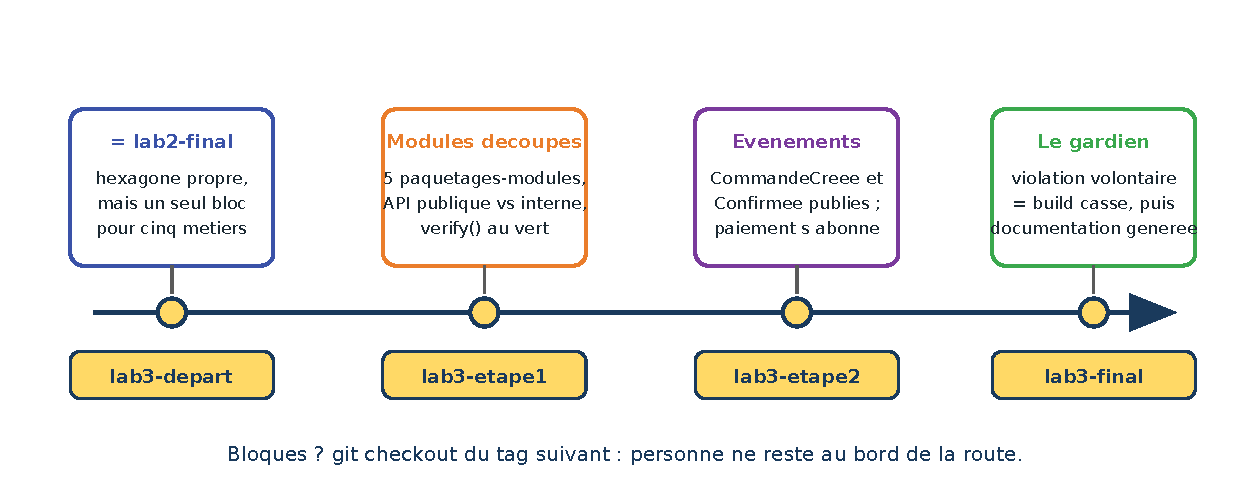
\includegraphics[width=0.80\linewidth]{figI_chemin_lab3}

{\scriptsize Point de départ : votre \texttt{lab2-final}. Les 8 tests (intégration + unitaires) restent verts — et un neuvième juge arrive : \texttt{verify()}.}
\end{frame}

\begin{frame}{Votre mission d'aujourd'hui}
{\scriptsize\begin{tabular}{p{0.20\linewidth}p{0.72\linewidth}}
\toprule
\textbf{Rôle} & \textbf{Propriétaire de module au Lab 3}\\
\midrule
Le Doyen & \texttt{commandes} — le module qui publie ; merges, tags, ADR\\
L'Huissier & \texttt{livraison} — l'API \texttt{AssignationLivreurs}, appelée en direct\\
Le Rédacteur & \texttt{catalogue} — et la documentation générée des modules\\
Le Notaire & \texttt{notifications} — les trois écouteurs, mêmes SMS qu'avant\\
L'Appariteur & \texttt{paiement} — le module né d'un événement, sans toucher aux autres\\
\bottomrule
\end{tabular}}
\vskip4pt
\begin{ucadrec}[Le livrable individuel de la séance]
{\small L'\textbf{Architecte du jour} signe l'\textbf{ADR n\textsuperscript{o}3 : « Comment tracer les frontières des modules ? »} — une page, deux alternatives sérieuses, deux conséquences négatives assumées.}
\end{ucadrec}
\end{frame}

\begin{frame}{L'essentiel de la séance}
\begin{ucadret}[À retenir]
{\footnotesize
\begin{itemize}
  \item La frontière qui manquait n'est pas technique : elle est \textbf{métier} — et se trouve en écoutant où \textbf{le vocabulaire change de sens}.
  \item Un \textbf{module} = une API publique au paquetage racine, des internes invisibles — et \textbf{Spring Modulith} transforme cette convention en \textbf{test} : violation = build cassé.
  \item Deux modes de collaboration : \textbf{appel direct} quand il faut une réponse (livraison), \textbf{événement} quand on informe (paiement, notifications) — et l'abonné naît sans toucher au publieur.
  \item Le modulith : 80\,\% des bénéfices d'organisation des microservices, 20\,\% de leur coût.
\end{itemize}}
\end{ucadret}
\begin{ucadfront}[La question qui ouvre la séance 4]
{\footnotesize La direction veut faire évoluer le calcul d'itinéraires avec l'écosystème Python — et le déployer sans redéployer tout SénResto. Un module peut-il \emph{quitter} le monolithe ? À quel prix ? Réponse au Lab 4 : l'extraction d'un microservice, pattern Strangler Fig.}
\end{ucadfront}
\end{frame}

\end{document}
